\section{HTTP Management Interface}
\label{section:http_mgt_iface}

All \glspl{cpe} researched have an \gls{http} Management Interface and it is enabled by default. The interface is a web service and as such, it is susceptible to a wide range of attacks if not properly implemented. Additionally, the management interface is accessible from the \gls{wan}-side on some devices. These factors make it an excellent attack vector.

This chapter analyses the different security aspects of the \gls{http} Management Interface as implemented on each \gls{cpe}. The problems are assessed and the impact discussed.

\subsection{Session}

The \gls{cpe} needs to keep the user authenticated while navigating through the management interface, this is generally done with \gls{http} Cookies \cite{rfc6265}.

By analyzing the requests made by the browser when accessing the interface of \glspl{cpe} 4, 6, and 7, it was found that the cookies contain only 8 to 10 characters, as shown on Figure \ref{figure:cpe_cookies}. It seems to be risky, but given that the sessions are short lived and that the \gls{http} server is slow, hardly a brute-force attack would succeed.

\begin{figure}[h]
    \centering
    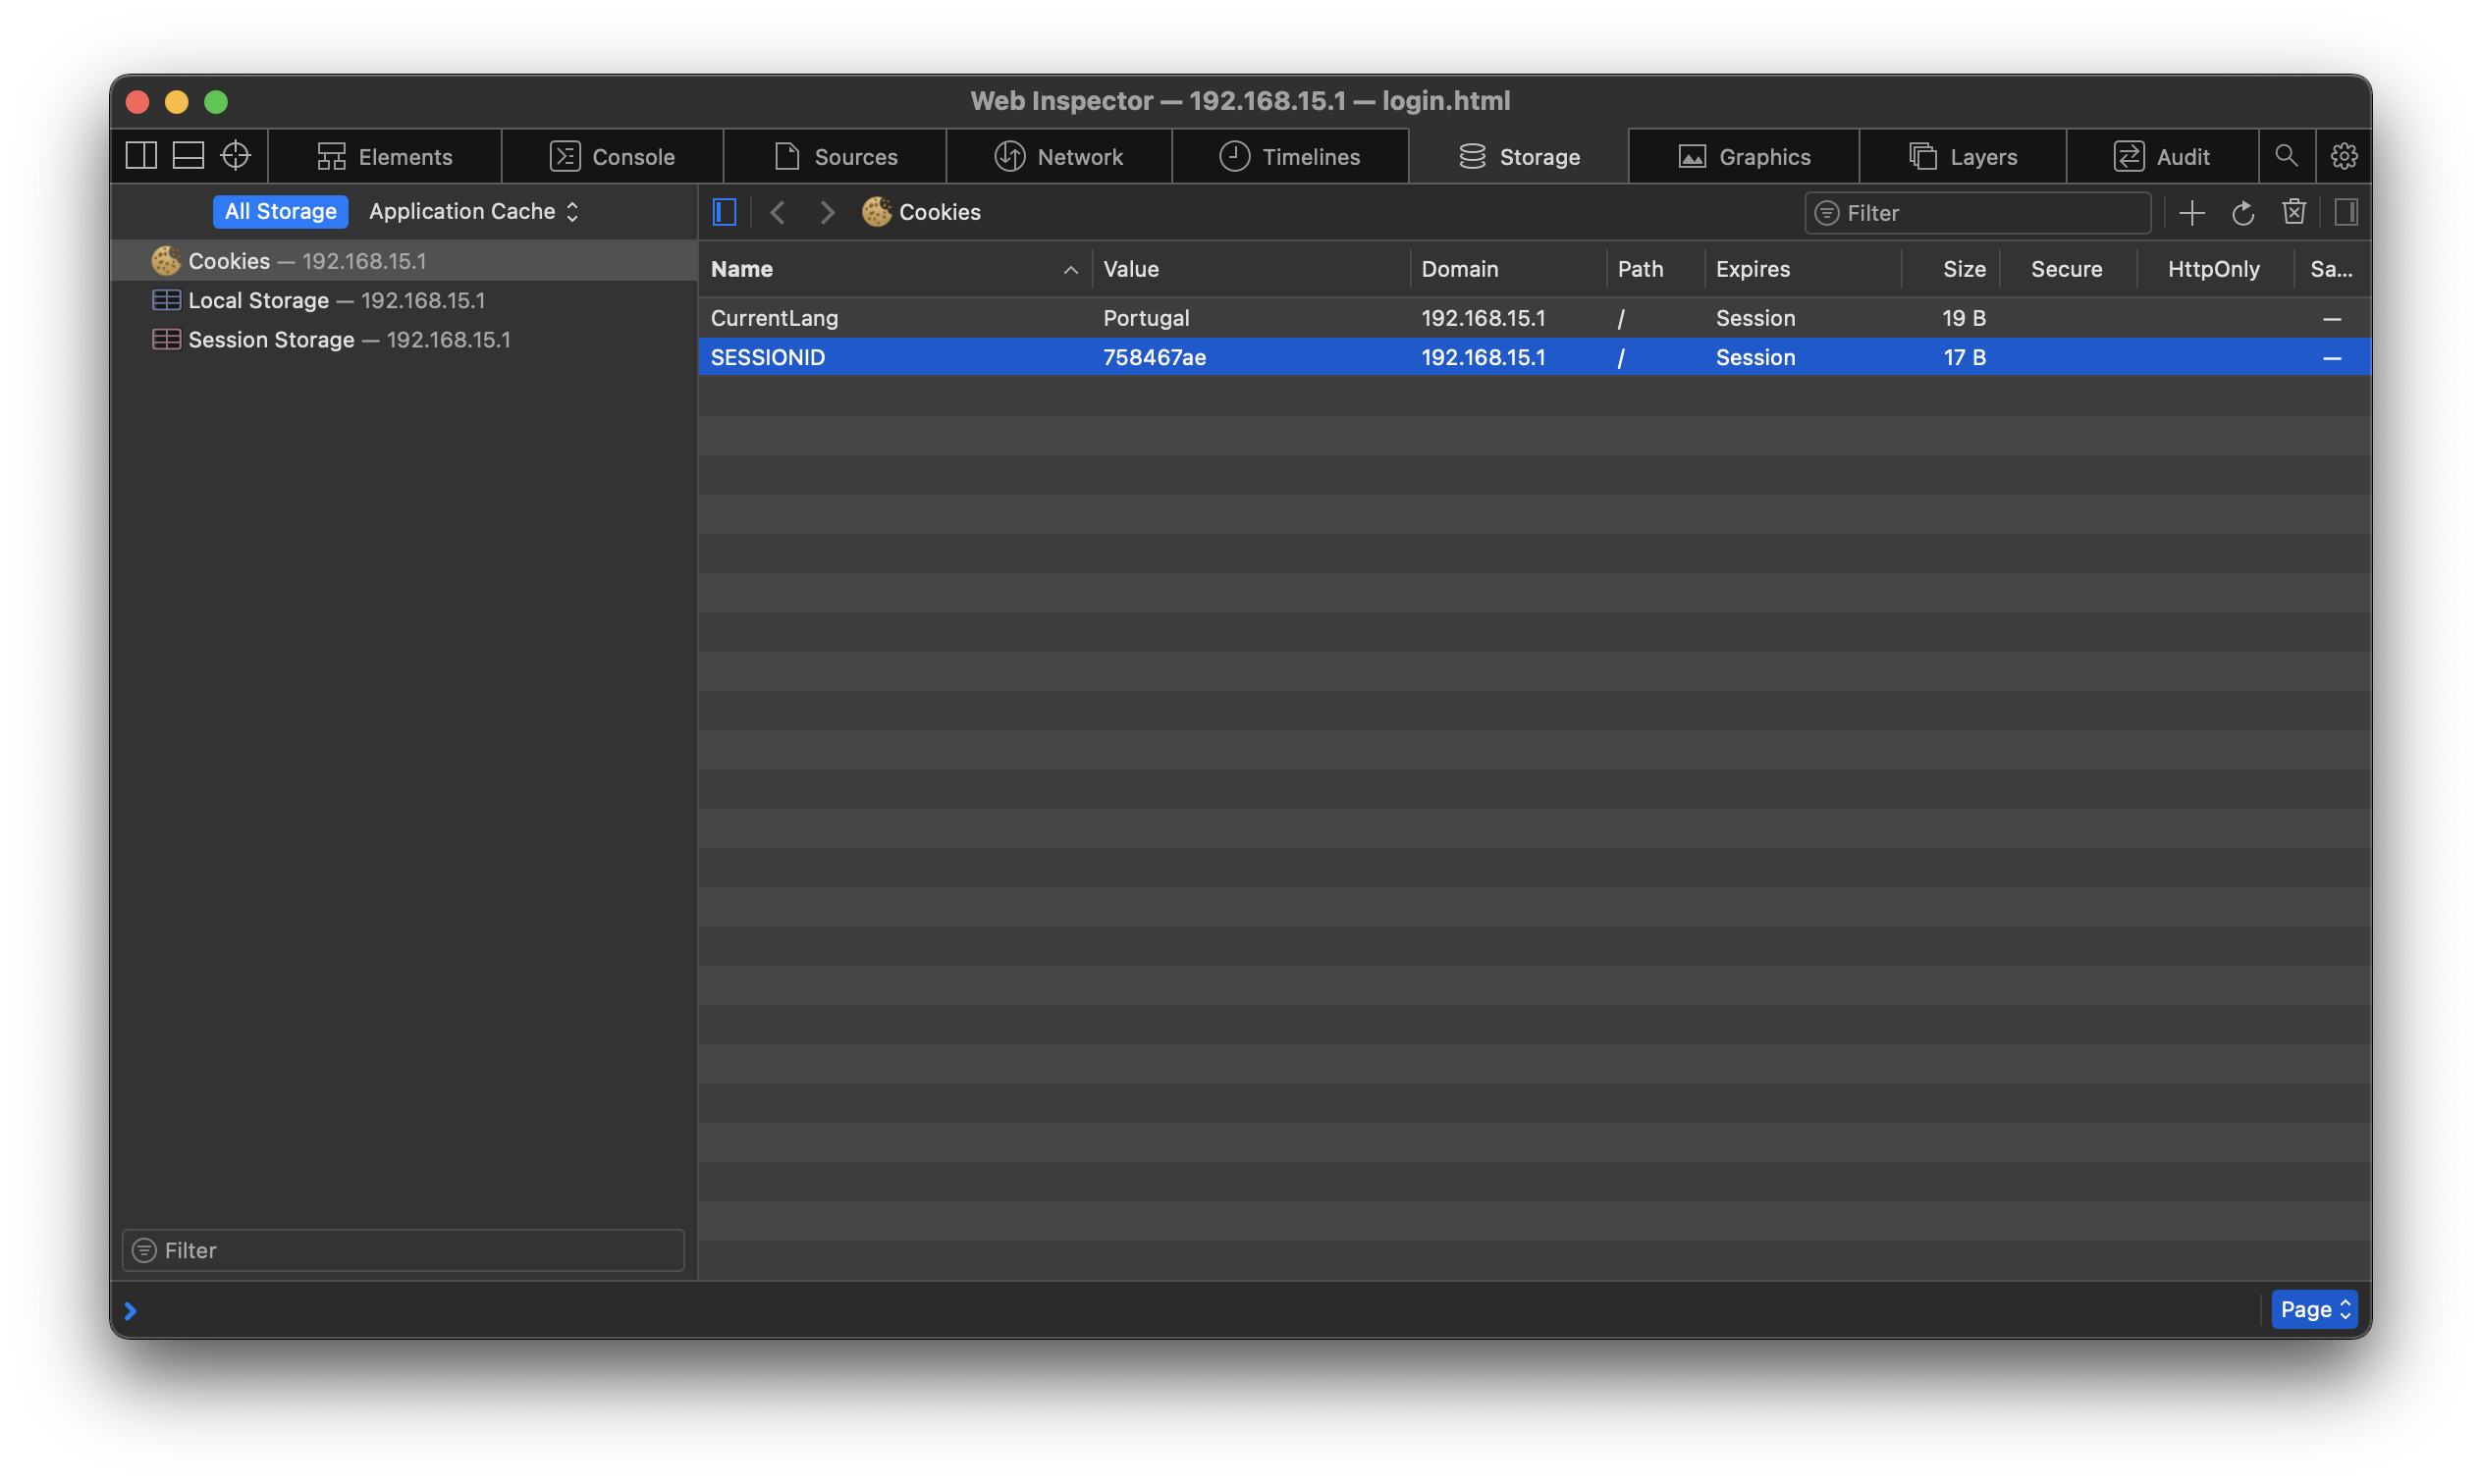
\includegraphics[width=\linewidth]{contents/http-management-interface-analysis/session/cpe-cookies.png}
    \caption{Cookies of the \gls{cwmp} \gls{http} Management Interface}
    \label{figure:cpe_cookies}
\end{figure}

Strangely, no cookie, authorization token, or any other method of keeping the user’s session was found on the captured requests of \glspl{cpe} 0 and 1. After performing some tests, it was identified that the \gls{cpe} authenticates the client based on its \gls{ip}. If another client on the network is able to hijack the \gls{ip} address of an authenticated user, it may gain access over the \gls{cpe}’s management interface.

\FloatBarrier

\subsection{Unauthenticated Routes}

On all \gls{cpe}s, at least two pages don’t require authentication for their contents to be viewed, the status and about pages. No other pages that can be accessed through the menu seem to work without proper authentication, but it is known that some pages of the web interface are not indexed and can only be accessed directly with their \gls{url}.

It is possible to make some hidden pages visible on \glspl{cpe} 0 and 1 by exporting the configuration file as previously mentioned, changing \texttt{PADRAO\_WIFI\_ONLY} from \texttt{0x0} to \texttt{0x1}, and reimporting the file. But to list all pages available on the \gls{http} Management Interface with certainty, the firmware image of each \gls{cpe} was expanded and inspected. 

To perform this operation, the binwalk tool was used. It takes a binary file and looks for different magic numbers of different file types, detecting which each segment of the file is. Then it is able to extract the individual segments and expand them.

By feeding the firmware images to binwalk, it was verified that \gls{cpe} 5 also carries the management interface of subsidiaries of the \gls{isp} in other countries. A configuration flag indicates which firmware should be used by the \gls{cpe} upon start. As the other management are not accessible without tampering with the device, their files were not inspected.

When testing the different \glspl{url} by using the file names, surprisingly, there was a serious finding on \gls{cpe} 5. The page responsible for importing and exporting configuration files doesn’t require authentication, as shown on Figure \ref{figure:unauthenticated_cpe_configuration_import}. Meaning that anyone that is able to send requests to the port 80/tcp is able to change any setting on the device, including the password of the management console, making null and void any kind of security on the management interfaces of the device.

\begin{figure}[h]
    \centering
    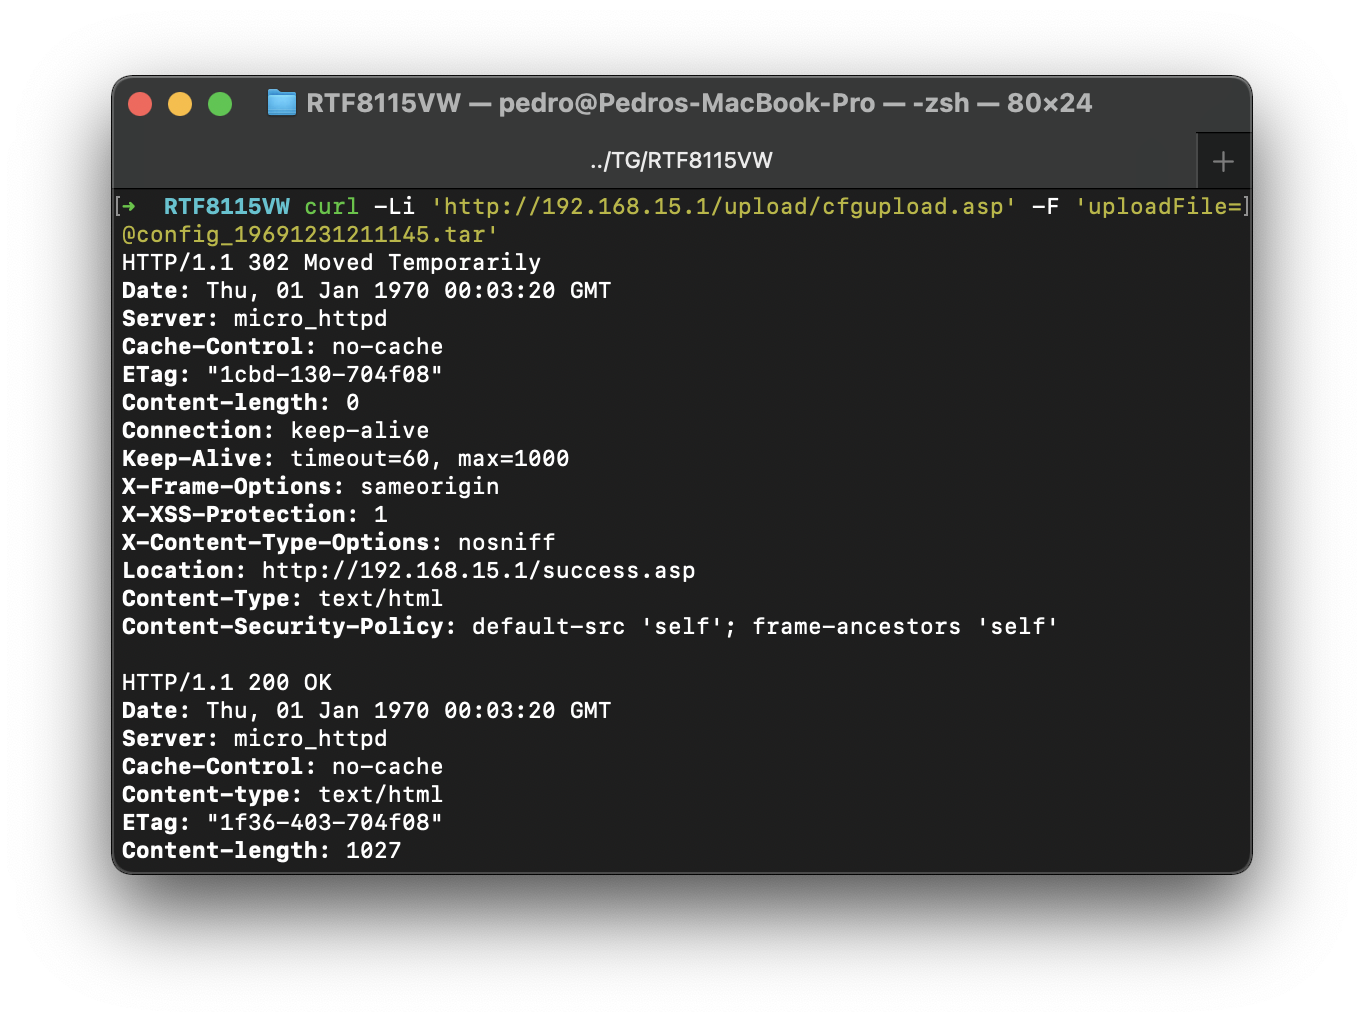
\includegraphics[width=\linewidth]{contents/http-management-interface-analysis/unauthenticated-routes/unauthenticated-cpe-configuration-import.png}
    \caption{Unauthenticated \gls{cwmp} Configuration Import}
    \label{figure:unauthenticated_cpe_configuration_import}
\end{figure}

\FloatBarrier

\subsection{Symbolic Links}

When exporting the configuration file, it was observed that \gls{cpe} 5 simply writes it in a path on the filesystem. Then the user can download it just by knowing its name, this is also true for any file under the specified directory.

Recently, it was discovered that some residential gateways have a vulnerability that allowed an attacker to access all files of the device’s file system by plugging a flash drive with a symbolic link to root on it \cite{cve-2020-5795}. This allowed the configuration files and password hashes to be recovered by accessing its sharing.

Similarly, a symbolic link to root was placed in the same folder as the configuration exports are stored. The result was that the \gls{http} server follows the symbolic link and allows every file on the equipment to be downloaded, as shown on Figure \ref{figure:cpe_symlink}.

\begin{figure}[h]
    \centering
    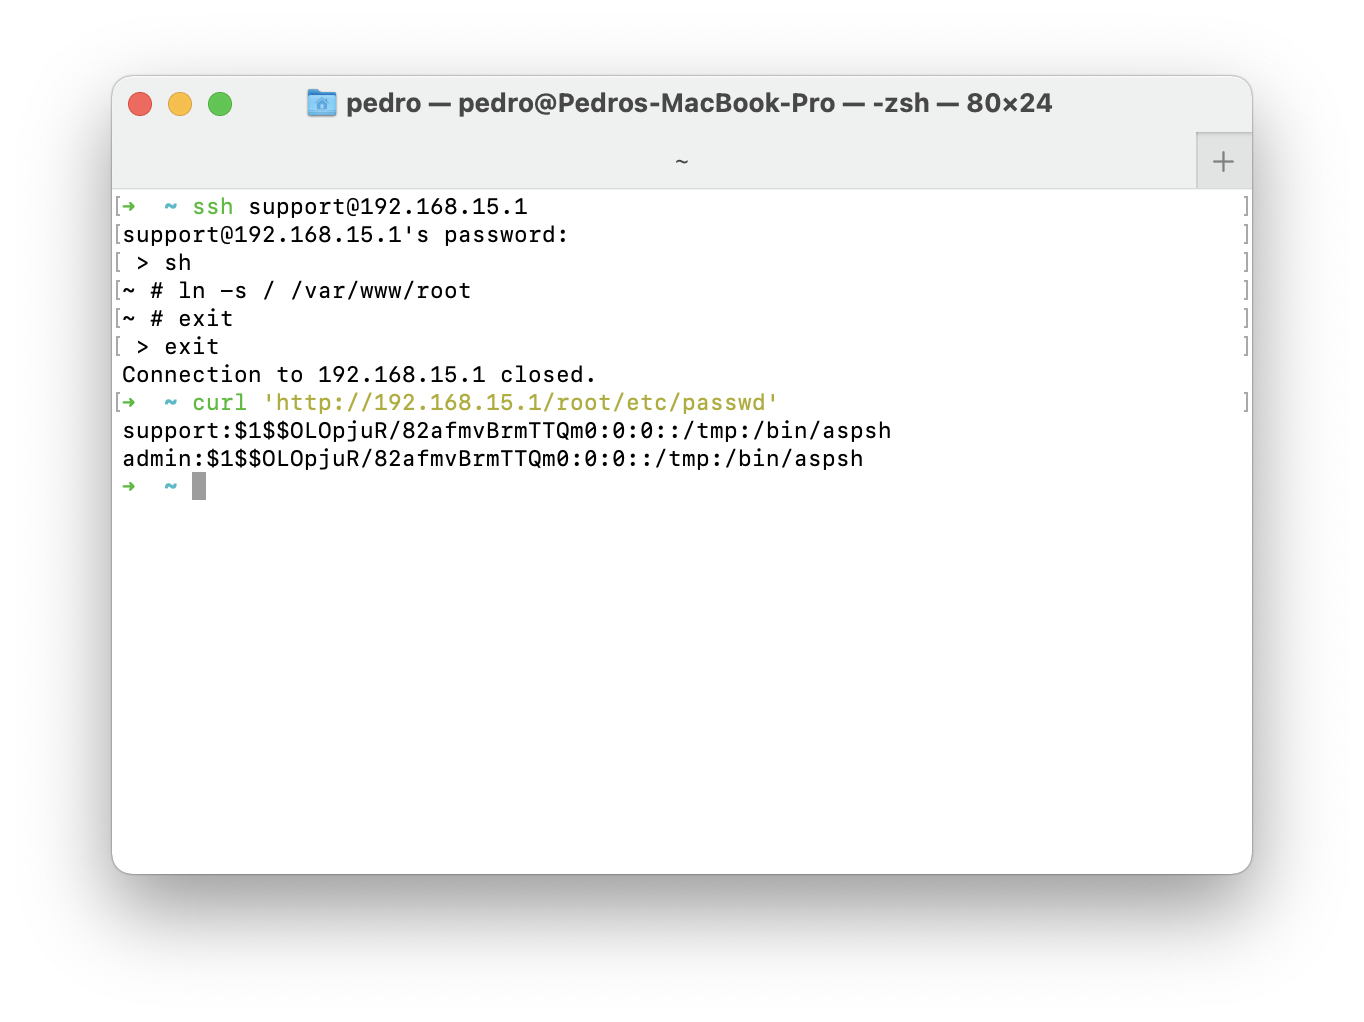
\includegraphics[width=\linewidth]{contents/http-management-interface-analysis/symbolic-links/cpe-http-management-interface-following-symbolic-link.png}
    \caption{\gls{cpe} \gls{http} Management Interface Following Symbolic Link}
    \label{figure:cpe_symlink}
\end{figure}

Although no way of injecting the malicious symbolic link on the device without requiring proper credentials was found, another vulnerability can be discovered in the future that would make this possible. Allowing an attacker to exploit it and gain access to all files on the device, including plaintext credentials.

\FloatBarrier

